\chapter{Scattering, Duality, and the Veneziano Amplitude}

\lectureoverview{Scattering reduces a collision to invariant data that can
be compared with experiment. For four identical particles those data may be
organized into the Mandelstam variables \(s,t,u\), only two of which are
independent. Ordinary particle exchange then suggests separate direct and
crossed channels. The Veneziano amplitude overturned that expectation: one
function contains both channel descriptions. The second half of the lecture
builds that function from two open strings that join, evolve as one
oscillating chain, and split again.}

\section{What a Theory Must Predict}

Fermionic strings solve two defects of the purely bosonic model: they admit
fermionic states and, after the appropriate projection, remove the tachyon.
Their critical spacetime dimension is ten rather than twenty-six. Extra
dimensions therefore remain, but their compactification is postponed. The
immediate subject is scattering.
\editorialnote{The tachyon-free statement refers to the consistent
superstring spectrum after the required projection; merely adding
world-sheet fermions is not by itself enough.}

Scattering is not necessarily the most interesting thing particles do. It is
simply the operation that an experiment can repeat cleanly. Send specified
particles toward one another, record the particles emerging from the
collision, and infer the dynamics hidden inside the interaction region. A
theory becomes quantitative when it supplies a complex amplitude
\begin{equation}
  \mathcal A(\hbox{incoming data}\to\hbox{outgoing data}),
\end{equation}
whose squared magnitude, together with the usual phase-space factors, gives
the probability for that outcome.

\begin{figure}[H]
  \centering
  
\includegraphics[width=0.72\textwidth]{lecture_06_figure_01.png}
  \caption{Incoming particles enter a black-box interaction region and
  outgoing particles emerge; time is drawn horizontally.}
  \lectureframe{00:02:35}
  \label{fig:l06-black-box}
\end{figure}

Particles also carry spin, charge, and species labels. To expose the
kinematics first, let us temporarily suppress everything except momentum.

\section{Four-Momentum and the All-Incoming Convention}

Write the four-momentum of one particle as
\begin{equation}
  k^\mu=(k^0,\mathbf k)=(E,\mathbf p).
\end{equation}
The lecture uses the mostly-plus metric, so
\begin{equation}
  k^2\equiv \mathbf p^2-E^2.
\end{equation}
The relativistic dispersion relation is therefore
\begin{equation}
  E^2-\mathbf p^2=m^2,
  \qquad
  k^2=-m^2.
  \label{eq:l06-mass-shell}
\end{equation}
Changing the spatial momentum changes the energy, but it does not move the
particle off its mass shell.

\begin{figure}[H]
  \centering
  
\includegraphics[width=0.66\textwidth]{lecture_06_figure_02.png}
  \caption{The mass-shell condition in the metric convention used
  throughout the lecture.}
  \lectureframe{00:05:56}
  \label{fig:l06-mass-shell}
\end{figure}

Consider two particles entering with momenta \(k_1,k_2\) and two leaving
with physical momenta \(q_3,q_4\). Conservation of energy and momentum is
one four-vector equation,
\begin{equation}
  k_1+k_2=q_3+q_4.
  \label{eq:l06-physical-conservation}
\end{equation}
It is convenient to assign an incoming momentum to every external line:
\begin{equation}
  k_3\equiv-q_3,
  \qquad
  k_4\equiv-q_4.
\end{equation}
Then
\begin{equation}
  k_1+k_2+k_3+k_4=0,
  \label{eq:l06-all-incoming}
\end{equation}
and every leg obeys \(k_i^2=-m_i^2\). The outgoing particles have negative
energy only in this bookkeeping convention; their physical energies remain
positive.

\begin{figure}[H]
  \centering
  
\includegraphics[width=0.68\textwidth]{lecture_06_figure_03.png}
  \caption{Physical outgoing momenta are reversed so that all four external
  momenta may be treated symmetrically as incoming.}
  \lectureframe{00:09:10}
  \label{fig:l06-all-incoming-board}
\end{figure}

At first the amplitude appears to be a function of sixteen components,
\(\mathcal A(k_1,k_2,k_3,k_4)\). Most of them are redundant. Go to the
center-of-mass frame, rotate the incoming momenta onto a chosen axis, and
assume for simplicity that all four particles have the same mass. The
incoming state is then fixed by one number, the center-of-mass energy. The
outgoing spatial momenta must be equal and opposite and have the same
magnitude as the incoming pair. Only their deflection angle \(\theta\)
remains. The process therefore has two independent kinematic variables:
\begin{equation}
  E_{\mathrm{cm}},
  \qquad
  \theta.
  \label{eq:l06-two-data}
\end{equation}

\section{Mandelstam Variables}

The two physical quantities in \eqref{eq:l06-two-data} should be expressible
without choosing a frame. With the all-incoming convention define
\begin{equation}
  -s=(k_1+k_2)^2,
  \qquad
  -t=(k_1+k_3)^2,
  \qquad
  -u=(k_1+k_4)^2.
  \label{eq:l06-mandelstam}
\end{equation}
In the center-of-mass frame the spatial parts of \(k_1+k_2\) cancel, hence
\begin{equation}
  s=E_{\mathrm{cm}}^2.
  \label{eq:l06-s-energy}
\end{equation}

For an outgoing physical momentum \(q_3=-k_3\),
\begin{equation}
  k_1+k_3=k_1-q_3
\end{equation}
is the momentum transferred from leg 1 to leg 3. For equal external masses,
with incoming spatial momentum magnitude \(p\),
\begin{equation}
  -t=2p^2(1-\cos\theta),
  \qquad
  -u=2p^2(1+\cos\theta).
  \label{eq:l06-tu-angle}
\end{equation}
Thus \(t\) and \(u\) carry the angular information measured by detectors.

\begin{figure}[H]
  \centering
  
\includegraphics[width=0.74\textwidth]{lecture_06_figure_04.png}
  \caption{The symmetric definitions of \(s,t,u\) in the all-incoming
  convention.}
  \lectureframe{00:26:20}
  \label{fig:l06-stu-board}
\end{figure}

Three symbols do not mean three independent data. Squaring
\eqref{eq:l06-all-incoming} and using \(k_i^2=-m^2\) gives
\begin{equation}
  s+t+u=4m^2
  \label{eq:l06-stu-constraint}
\end{equation}
for equal masses. Once \(s\) and \(t\) are known, \(u\) is fixed.

\begin{classroomqa}
\audiencequestion{Could the vacuum slow a freely moving particle, rather
like friction? \lecturetimestamp{00:27:17}}
\lecturerresponse{Not in a translation-invariant vacuum. There is nowhere
for the missing momentum to go, so momentum conservation forbids such
friction. One can imagine a medium or a different vacuum that selects a
preferred rest frame, but that is not the vacuum being used here.}
\end{classroomqa}

\begin{classroomqa}
\audiencequestion{Why must the two outgoing particles have equal
energies? \lecturetimestamp{00:27:54}}
\lecturerresponse{In the center-of-mass frame their spatial momenta must be
equal and opposite. For the equal-mass process under discussion, equal
momentum magnitudes give equal energies through
\(E^2=p^2+m^2\). If the outgoing masses differed, that last conclusion
would have to be modified.}
\end{classroomqa}

\section{Direct and Crossed Channels}

A simple point-particle diagram lets particles 1 and 2 form an intermediate
particle of mass \(M\), which then decays into 3 and 4. Up to numerator
factors and the pole prescription, its characteristic dependence is
\begin{equation}
  \mathcal A_s\sim\frac{g^2}{s-M^2}.
  \label{eq:l06-s-channel}
\end{equation}
This is the direct, or \(s\)-channel, process. Turning the connectivity
sideways gives exchange between the two external lines,
\begin{equation}
  \mathcal A_t\sim\frac{g^2}{t-M^2},
  \label{eq:l06-t-channel}
\end{equation}
the crossed, or \(t\)-channel, process. A third connectivity gives
\begin{equation}
  \mathcal A_u\sim\frac{g^2}{u-M^2}.
  \label{eq:l06-u-channel}
\end{equation}

\begin{figure}[H]
  \centering
  
\includegraphics[width=0.72\textwidth]{lecture_06_figure_05.png}
  \caption{Direct production through an intermediate state and the
  corresponding pole \(g^2/(s-M^2)\); the crossed connectivity is being
  assembled on the same board.}
  \lectureframe{00:30:50}
  \label{fig:l06-channel-board}
\end{figure}

The distinction is physical. At this crude scalar level,
\eqref{eq:l06-s-channel} depends on collision energy but not on angle. The
compound state has forgotten the incident direction before it decays, so its
decay is isotropic. The exchange amplitude depends on momentum transfer and
therefore on angle; a light exchanged particle strongly favors small
deflection. Spin would add further angular dependence, but the pole
structure is already visible.

\begin{classroomqa}
\audiencequestion{Does the missing \(u\)-channel produce a third
term? \lecturetimestamp{00:34:47}}
\lecturerresponse{Yes, whenever the particle identities and couplings permit
that connectivity. One then includes a term with a pole at \(u=M^2\). It is
not a new independent kinematic variable, because
\(s+t+u=4m^2\), but it is a distinct channel diagram.}
\end{classroomqa}

\section{One Function, Two Channel Descriptions}

A single pole is a poor model of meson scattering. Two mesons can form many
resonances, with a tower of masses and angular momenta. The first response in
the 1960s was to add more \(s\)-channel poles, more \(t\)-channel poles, and
the allowed \(u\)-channel poles. Then a much more economical function was
found. In the lecture's units, where the linear Regge trajectory and its
intercept have been absorbed into \(s\) and \(t\), it is
\begin{equation}
  \mathcal A_{\mathrm V}(s,t)
  \propto
  \frac{\Gamma(-s)\Gamma(-t)}{\Gamma(-s-t)}.
  \label{eq:l06-veneziano}
\end{equation}
The gamma function continues the factorial:
\begin{equation}
  \Gamma(n)=(n-1)!
\end{equation}
at positive integers.

\begin{figure}[H]
  \centering
  
\includegraphics[width=0.68\textwidth]{lecture_06_figure_06.png}
  \caption{The Veneziano amplitude written as a symmetric ratio of gamma
  functions.}
  \lectureframe{00:42:25}
  \label{fig:l06-veneziano-board}
\end{figure}

The poles of \(\Gamma(-s)\) reproduce an infinite tower of direct-channel
resonances. Yet the same expression is symmetric under \(s\leftrightarrow
t\), so its \(\Gamma(-t)\) poles give a crossed-channel expansion. These are
not two separately added contributions. One analytic function admits either
description. This is the old idea of duality between direct-channel
resonances and crossed-channel exchanges.

\begin{classroomqa}
\audiencequestion{How can one amplitude contain both channel sums without
adding them? \lecturetimestamp{00:43:32}}
\lecturerresponse{That is precisely the surprise. Expanding the function
near its \(s\)-channel poles organizes it as direct resonances; expanding it
near its \(t\)-channel poles organizes the same function as exchanges. A
microscopic model is needed to explain why those two readings are the same,
and the model is an interacting string.}
\end{classroomqa}

\section{A Strip Swept Out by an Open String}

Parameterize an open string by
\begin{equation}
  0\leq\sigma\leq\pi.
\end{equation}
The label \(\sigma\) is not a spacetime position. The embedding
\(X^\mu(\sigma,\tau)\) tells us where that labeled point lies in spacetime,
while \(\tau\) measures evolution. A point particle sweeps out a worldline;
the moving string sweeps out a two-dimensional worldsheet. In the free
theory each embedding coordinate obeys
\begin{equation}
  \frac{\partial^2X^\mu}{\partial\tau^2}
  -
  \frac{\partial^2X^\mu}{\partial\sigma^2}
  =0.
  \label{eq:l06-wave-equation}
\end{equation}

\begin{figure}[H]
  \centering
  
\includegraphics[width=0.70\textwidth]{lecture_06_figure_07.png}
  \caption{The wave equation governing each free string coordinate on the
  worldsheet strip.}
  \lectureframe{00:49:10}
  \label{fig:l06-wave-equation-board}
\end{figure}

For the scattering construction it is useful not to take the continuum
limit too soon. Replace each string by \(n\) mass points joined by springs.
The worldsheet becomes a dense collection of nearby worldlines, and its
normal modes are ordinary harmonic oscillators. Two incoming chains can
touch at their endpoints. At that event a new spring joins them, they evolve
for a time \(\tau\) as one longer chain, and later a spring breaks so that two
outgoing chains emerge.

\begin{figure}[H]
  \centering
  
\includegraphics[width=0.72\textwidth]{lecture_06_figure_08.png}
  \medskip

  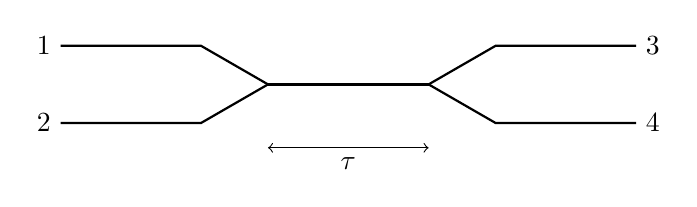
\begin{tikzpicture}[x=0.85cm,y=0.70cm]
    \draw[thick] (0,2.2) -- (2.1,2.2) -- (3.1,1.5);
    \draw[thick] (0,0.8) -- (2.1,0.8) -- (3.1,1.5);
    \draw[thick] (3.1,1.5) -- (5.5,1.5);
    \draw[thick] (5.5,1.5) -- (6.5,2.2) -- (8.6,2.2);
    \draw[thick] (5.5,1.5) -- (6.5,0.8) -- (8.6,0.8);
    \draw[<->] (3.1,0.35) -- node[below] {\(\tau\)} (5.5,0.35);
    \node[left] at (0,2.2) {1};
    \node[left] at (0,0.8) {2};
    \node[right] at (8.6,2.2) {3};
    \node[right] at (8.6,0.8) {4};
  \end{tikzpicture}
  \caption{Two discretized open strings touch, form one intermediate string
  for a duration \(\tau\), and split. The source frame preserves the
  spring-and-worldline construction; the schematic isolates its
  connectivity.}
  \lectureframe{00:51:25}
  \label{fig:l06-string-joining}
\end{figure}

The two strings are drawn adjacent in parameter space only. Their spacetime
positions need not be adjacent until the endpoint coordinates actually
coincide. Reparameterization freedom lets the joining and splitting events
be placed at convenient positions on the diagram; this geometric freedom
will become conformal symmetry in the next lecture.

\section{The Oscillator Calculation in Slow Motion}

Let the first chain have coordinates \(x_1,\ldots,x_n\), and the second
\(x_{n+1},\ldots,x_{2n}\). Their center-of-mass coordinates are
\begin{equation}
  X_{\mathrm{cm}}^{(1)}
  =\frac1n\sum_{a=1}^{n}x_a,
  \qquad
  X_{\mathrm{cm}}^{(2)}
  =\frac1n\sum_{a=n+1}^{2n}x_a.
  \label{eq:l06-chain-centers}
\end{equation}
A chain with definite momentum \(k_1\) has a center-of-mass plane wave
multiplied by an internal oscillator ground state:
\begin{align}
  \Psi_1
  &=
  e^{ik_1\cdot X_{\mathrm{cm}}^{(1)}}
  \psi_0(x_1,\ldots,x_n),
  \\
  \Psi_2
  &=
  e^{ik_2\cdot X_{\mathrm{cm}}^{(2)}}
  \psi_0(x_{n+1},\ldots,x_{2n}).
  \label{eq:l06-two-wavefunctions}
\end{align}
The factors \(\psi_0\) depend on relative coordinates, not on the common
translation of an entire chain. Because the incoming strings are initially
separate quantum systems,
\begin{equation}
  \Psi_{\mathrm{in}}=\Psi_1\Psi_2.
  \label{eq:l06-product-state}
\end{equation}

\begin{figure}[H]
  \centering
  
\includegraphics[width=0.76\textwidth]{lecture_06_figure_09.png}
  \caption{The two momentum plane waves and their internal oscillator
  ground-state factors, written in separate colors.}
  \lectureframe{00:58:05}
  \label{fig:l06-wavefunctions-board}
\end{figure}

Joining selects the part of this wavefunction for which the two endpoint
coordinates agree:
\begin{equation}
  x_n=x_{n+1}.
  \label{eq:l06-endpoint-contact}
\end{equation}
At that instant the other coordinates are unchanged. The selected state is
then evolved with the Hamiltonian \(H_{\mathrm{joined}}\) of the single
longer chain:
\begin{equation}
  \Psi(\tau)
  =
  e^{-iH_{\mathrm{joined}}\tau}\Psi(0).
  \label{eq:l06-time-evolution}
\end{equation}
Finally one takes its overlap with a product of outgoing string states
carrying momenta \(q_3,q_4\).

\begin{figure}[H]
  \centering
  
\includegraphics[width=0.76\textwidth]{lecture_06_figure_10.png}
  \caption{The two-chain wavefunction immediately before the endpoint
  coincidence is imposed.}
  \lectureframe{00:58:55}
  \label{fig:l06-endpoint-board}
\end{figure}

The calculation is lengthy but not mysterious. Every internal coordinate
can be decomposed into oscillator modes, so the joining overlap, time
evolution, and final projection reduce to Gaussian oscillator algebra.
What remains unfixed is the lifetime \(\tau\) of the joined string.

\begin{classroomqa}
\audiencequestion{Are the black and red wavefunctions added or
multiplied? \lecturetimestamp{01:02:26}}
\lecturerresponse{Multiplied. The tensor-product state of two independent
systems is represented in the coordinate basis by the product of their
wavefunctions. Addition would describe a superposition of alternatives, not
the simultaneous presence of both incoming strings.}
\end{classroomqa}

\begin{classroomqa}
\audiencequestion{Why integrate over the intermediate time
\(\tau\)? \lecturetimestamp{01:04:04}}
\lecturerresponse{The joined string is not assigned a fixed lifetime.
Feynman's rule is to sum amplitudes over all allowed histories. In this
description the remaining continuous history parameter is the time between
joining and splitting, so the sum becomes an integral over
\(0\leq\tau<\infty\).}
\end{classroomqa}

\section{From Propagation Time to the Beta Function}

After evaluating the oscillator overlaps, the result can be organized as
\begin{equation}
  \mathcal A(s,t)
  \propto
  \int_0^\infty d\tau\,
  e^{\tau(s+1)}
  \bigl(1-e^{-\tau}\bigr)^{-t-1}
  e^{-\tau}.
  \label{eq:l06-tau-integral}
\end{equation}
The final \(e^{-\tau}\) is kept visible because it is the Jacobian needed in
the next step. Equivalently, the first and last exponentials combine to
\(e^{s\tau}\).

\begin{figure}[H]
  \centering
  
\includegraphics[width=0.76\textwidth]{lecture_06_figure_11.png}
  \caption{The propagation-time integrand after the oscillator calculation;
  the separate \(e^{-\tau}\) factor supplies the change-of-variables
  Jacobian.}
  \lectureframe{01:06:45}
  \label{fig:l06-tau-integral-board}
\end{figure}

Now set
\begin{equation}
  z=e^{-\tau},
  \qquad
  dz=-e^{-\tau}\,d\tau.
  \label{eq:l06-z-substitution}
\end{equation}
As \(\tau\) runs from \(0\) to \(\infty\), \(z\) runs from \(1\) to \(0\).
The minus sign reverses the limits, giving
\begin{equation}
  \mathcal A(s,t)
  \propto
  \int_0^1
  z^{-s-1}(1-z)^{-t-1}\,dz.
  \label{eq:l06-beta-integral}
\end{equation}

\begin{figure}[H]
  \centering
  
\includegraphics[width=0.74\textwidth]{lecture_06_figure_12.png}
  \caption{The substitution \(z=e^{-\tau}\) exposes the Euler beta
  integral.}
  \lectureframe{01:08:49}
  \label{fig:l06-beta-integral-board}
\end{figure}

This integral is defined directly where its endpoints converge and
elsewhere by analytic continuation. It is the Euler beta function:
\begin{equation}
  B(-s,-t)
  =
  \frac{\Gamma(-s)\Gamma(-t)}{\Gamma(-s-t)}.
  \label{eq:l06-beta-gamma}
\end{equation}

\begin{figure}[H]
  \centering
  
\includegraphics[width=0.72\textwidth]{lecture_06_figure_13.png}
  \caption{The board identifies the transformed integral with
  \(B(-s,-t)\) and begins restoring its gamma-function form.}
  \lectureframe{01:12:24}
  \label{fig:l06-beta-gamma-board}
\end{figure}

The channel symmetry is now elementary. Under \(z\mapsto1-z\),
\begin{equation}
  \int_0^1 z^{-s-1}(1-z)^{-t-1}\,dz
  =
  \int_0^1 z^{-t-1}(1-z)^{-s-1}\,dz.
\end{equation}
Thus \(\mathcal A(s,t)=\mathcal A(t,s)\). A process constructed as two
strings joining and later splitting automatically contains the crossed
description as well.
\editorialnote{The lecture suppresses the Regge slope and intercept in the
arguments of the beta function. In standard notation one replaces \(s,t\)
by the corresponding linear trajectories \(\alpha(s),\alpha(t)\). The
duality and the change-of-variables argument are unchanged.}

\begin{classroomqa}
\audiencequestion{The gamma-function ratio resembles factorial expressions
in combinatorics. Is there a direct physical counting
interpretation? \lecturetimestamp{01:13:22}}
\lecturerresponse{At integer arguments the beta function is related to a
ratio such as \(n!\,m!/(n+m)!\), but no combinatorial mechanism is being
asserted here. The same special function happens to arise from the
worldsheet integral; this resemblance was not the route by which the
amplitude was found.}
\end{classroomqa}

The still-hidden reason why one worldsheet can be read in both channels is
conformal symmetry. It permits the sheet to be stretched like taffy without
changing the amplitude, turning a long direct-channel propagation region
into a crossed-channel exchange picture. That geometric explanation is
deferred to the next lecture.

\section{What the Scattering Test Established}
\enlargethispage{3\baselineskip}
\begingroup
\setlength{\medskipamount}{3pt plus 1pt minus 1pt}

The discrete joining picture prompted a final cluster of questions.

\begin{classroomqa}
\audiencequestion{If two chains of \(n\) constituents join at their
endpoints, is the result \(2n-1\), and could that change fermion
parity? \lecturetimestamp{01:16:16}}
\lecturerresponse{In the hadronic endpoint picture the touching endpoint
pair may be regarded as a particle-antiparticle pair that annihilates, so
the count is reduced by two, not one. In the continuum limit the finite
difference between \(2n\) and \(2n-2\) is immaterial, but preserving fermion
parity is not. The lattice constituents are only a regulator for the
continuous string, not literal fundamental beads.}
\end{classroomqa}

\begin{classroomqa}
\audiencequestion{Will the later discussion continue into the full
mathematics of superstrings? \lecturetimestamp{01:18:05}}
\lecturerresponse{Only selected consequences will be used. The immediate
route is through worldsheet symmetry and compactification, followed by a
different starting point developed in the mid-1990s: M-theory. Its purpose
is to reach the same physics from a viewpoint in which several otherwise
complicated features become transparent.}
\end{classroomqa}

\begin{classroomqa}
\audiencequestion{Was this joining rule only a clue from meson
collisions? \lecturetimestamp{01:20:02}}
\lecturerresponse{Meson scattering supplied the historical clue, but the
rule is general for open strings. The same topology describes collisions of
open-string photons and other open-string states. Two closed strings join
and split by an analogous construction, with a closed string in the
intermediate region.}
\end{classroomqa}

\begin{classroomqa}
\audiencequestion{Does the calculation apply only when the string states are
fermions? \lecturetimestamp{01:20:56}}
\lecturerresponse{No. The original Veneziano calculation belongs to the
bosonic open string. Superstrings require additional fermionic degrees of
freedom and modify details of the integrand, but the joining, propagation,
projection, and worldsheet-duality logic remains closely analogous.}
\end{classroomqa}

Finding a spin-one or spin-two state in the oscillator spectrum was
suggestive, but not decisive. Their scattering amplitudes supplied the
stronger test. Photon amplitudes obey the identities associated with charge
conservation and gauge invariance; graviton amplitudes obey the corresponding
constraints of a massless spin-two field. The string states passed these
tests in interactions with massive and massless states and with one another.
That is why the photon and graviton labels became physical identifications
rather than guesses based only on polarization counting.
\editorialnote{In modern language these tests are encoded in decoupling of
unphysical polarizations, gauge Ward identities, and the universal
low-energy coupling of the massless spin-two state.}

\begin{classroomqa}
\audiencequestion{Where does electric charge itself come from in the string
description? \lecturetimestamp{01:24:03}}
\lecturerresponse{That question is left open at the end of the lecture. Its
answer requires the internal and endpoint structure of the string theory,
which has not yet been introduced, so it belongs to the discussion that
follows rather than to this scattering derivation.}
\end{classroomqa}
\endgroup
